
\begin{mydef}
La classe $\p$ contient tous les problèmes de décision pour lesquelles on peut trouver une réponse avec une machine de Turing en un nombre d'étapes borné par une fonction polynomiale en la taille des entrées.
\end{mydef}
\begin{mydef}
La classe $\np$ contient tous les problèmes de décision pour lesquelles on peut vérifier une solution correcte avec une machine de Turing en un nombre d'étapes borné par une fonction polynomiale en la taille des entrées.
\end{mydef}
\begin{mydef}
Un problème $\pi$, de décision ou d'optimisation, est $ \np-difficile$ si tous les problèmes de la classe $\np$ admettent une réduction polynomiale vers $\pi$. 
\end{mydef}


\wsrp combine la complexité des problèmes d'ordonnancement \cite{Blazewicz1983,Lageweg1982} : ordonnancement de projet à compétences multiples (Multi-skill Project Scheduling Problem, Tehcnician and Task Scheduling Problem), séquençage et ordonnancement de tâches (Sequencing and Scheduling Problem) \cite{Lawler1993}, ordonnancement de projet avec contraintes de ressources (Resources Constrained Project Scheduling Problem) et des problèmes de tournée de véhicule \cite{Lenstra2013,Tsitsiklis1992} : problème de tournée de véhicule avec fenêtre de temps (Vehicule Routing Problem with Time Windows), problème de tournée de véhicule avec fenêtre de temps, dépendance temporelle (Vehicle Routing Problem with Time Windows and Time Dependancies) et Traveling Salesman Problem with Time Windows. Nous allons avoir besoin de définir quelques problèmes  avant de pouvoir définir la complexité de \wsrp.









%\probdef{Un graphe $G=(V,E,\omega)$ non orienté et M < |V|.}{Trouver $m\leq M$ cycles disjoints de coût Min couvrant V}{Vehicule Routing Problem}{VRP}{def:VRP}


\indent 


\begin{comment}
La Figure~\ref{Fig:Complexite} montre le lien entre les problèmes défini plus haut.


\begin{figure}[H]
\centering
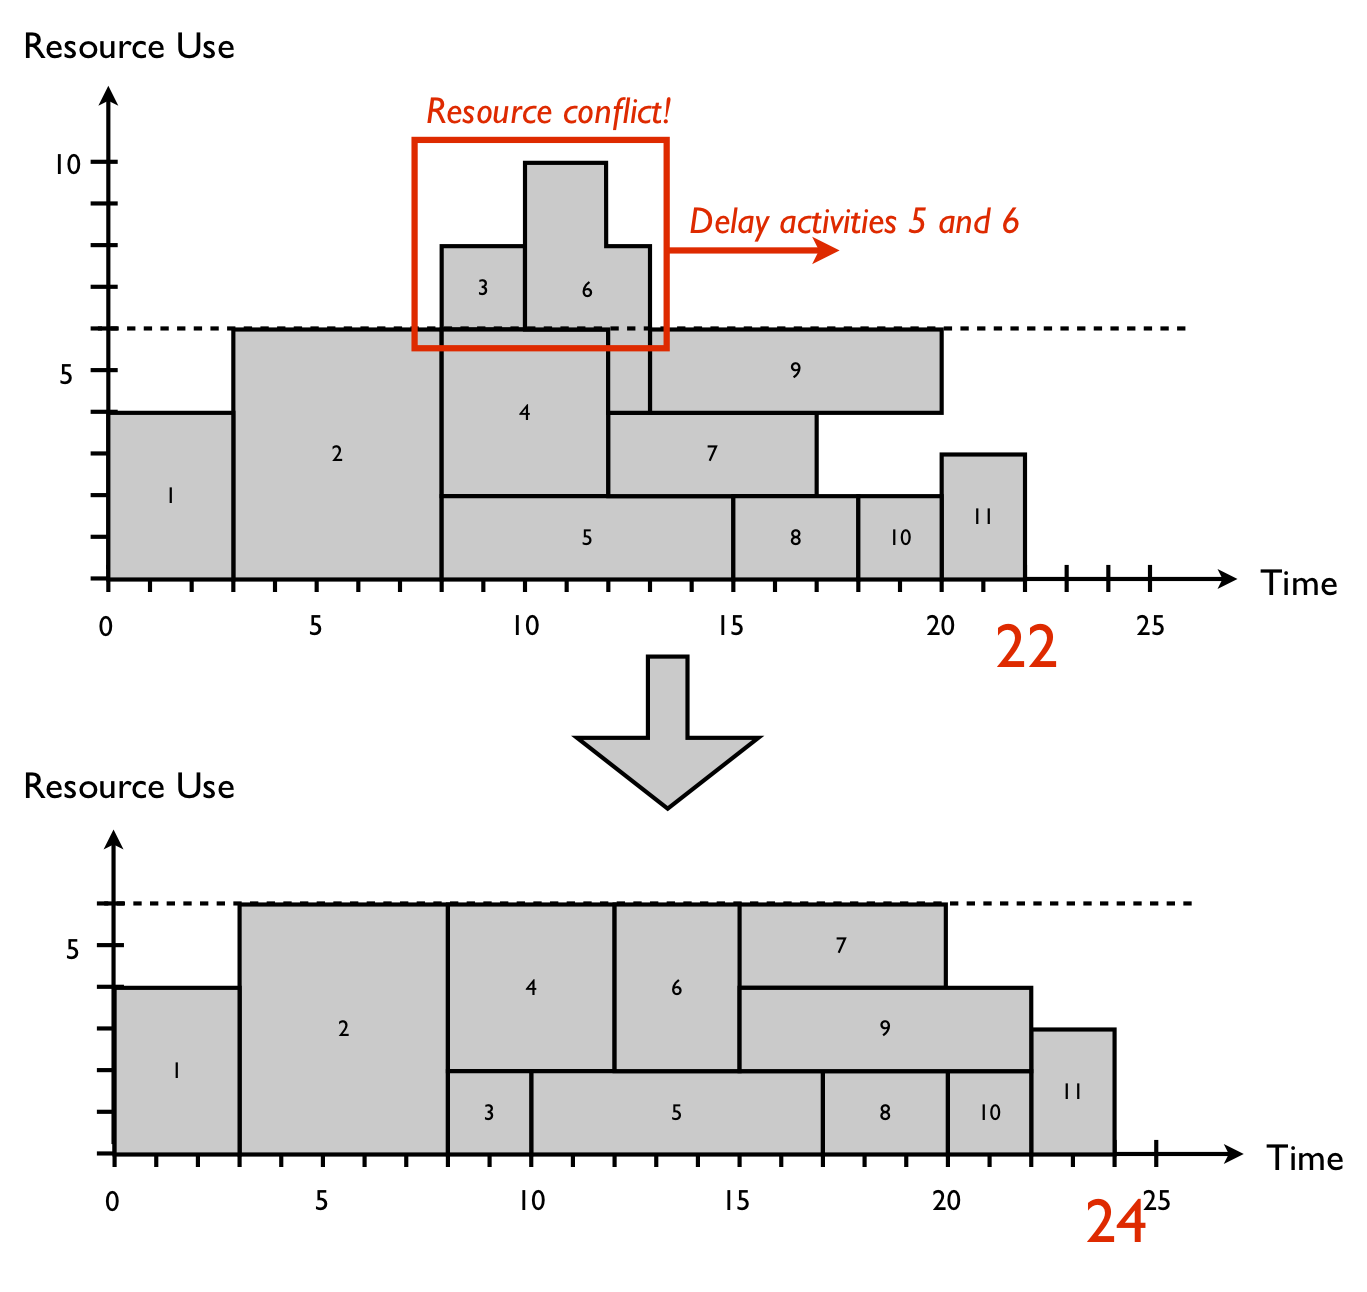
\includegraphics[scale=0.4]{RCPSP}
\caption{\label{RCPSP} Exemple de problème d'ordonnancement de projet avec contrainte de ressources.La ligne en pointillé représente la contrainte de ressources, l'ordonnancement du bas est une solution réalisable alors que celui du haut est une solution qui ne respecte pas la contrainte de ressource}
\end{figure}
\end{comment}

\begin{comment}



\begin{defPb}{Le problème d'ordonnancement de techniciens et de tâches}{Technician and Task Scheduling Problem}

\end{defPb}



\begin{defPb}{Le problème d'ordonnancement et de routage de techniciens}{Technician Routing and Scheduling Problem} \cite{zamorano2017branch} est majoritairement présent dans le domaine de la maintenance d'équipement et d'installation dans des bâtiments.
\end{defPb}

\begin{defPb}{Le problème d'Assistance à Domicile} {Home Care Problem} vise à assisté des personnes âgées ou handicapée pour effectuer des tâches quotidiennes (faire les courses, se préparer à manger, etc). \cite{akjiratikarl2007pso}
\end{defPb}

\begin{defPb}{Le problème de planning d'infirmière} {Nurse Scheduling/Nurse Rostering Problem} est un problème qui possède beaucoup de contraintes souvent séparé en contraintes "molles" (soft constraint) qui peuvent être violées mais cela à un coût et contraintes "dures" (hard constraint) qui ne peuvent pas être violées \cite{Trilling2007}. L.  
\end{defPb}



\begin{defPb}{Le problème de Soins Infirmiers à Domicile}{Home Health Care Problem} est une extension du problème de planning d'infirmière. En effet en plus de fournir un planning qui respecte les préférences des infirmières, il faut associé à chaque infirmière une tournée qui minimise le temps de trajet entre chaque visite. On peut le voir aussi comme une variante de \trsp \cite{Bertels2006,Rasmussen2010}.
\end{defPb}

\begin{defPb}{Le problème de Planning et Routage de Personnel de Sécurité}{Security Personal Routing and Rostering} est un problème possède à la fois la dimension de routage (Multi Depot Vehicule Routing Problem) et la dimension d'ordonnancement (Multi-skill Project Scheduling Problem) et pour chacune de ces dimensions le problème est assez contraint. Le problème est assez similaire au problème de Soins Infirmiers à Domicile mais l'horizon du planning est beaucoup plus long \cite{misir2011security}.
\end{defPb}

\begin{defPb}{Le problème de Répartition de Main-d’œuvre}{Manpower Allocation}\cite{lim2004}
\end{defPb}

\begin{defPb}{Le problème de ramassage/récolte et livraison}{Pick-up and Delivery Problem} \cite{Ropke2005}
\end{defPb}

\begin{figure}[H]
\centering
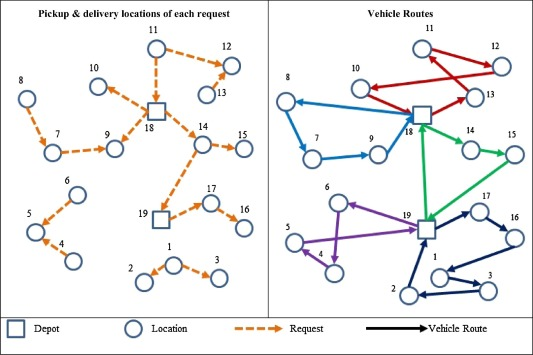
\includegraphics[scale=0.8]{PDP}
\caption{Exemple de routage pour le \pdp\label{fig:PDP}}
\end{figure}
\end{comment}